\documentclass[format=acmtog]{acmart}

\usepackage{amssymb,amsmath}
\usepackage{ifxetex,ifluatex}
\usepackage{fixltx2e} % provides \textsubscript
\ifnum 0\ifxetex 1\fi\ifluatex 1\fi=0 % if pdftex
  \usepackage[T1]{fontenc}
  \usepackage[utf8]{inputenc}
\else % if luatex or xelatex
  \usepackage{unicode-math}
  \defaultfontfeatures{Ligatures=TeX,Scale=MatchLowercase}
\fi
% use upquote if available, for straight quotes in verbatim environments
\IfFileExists{upquote.sty}{\usepackage{upquote}}{}
% use microtype if available
\IfFileExists{microtype.sty}{%
\usepackage[]{microtype}
\UseMicrotypeSet[protrusion]{basicmath} % disable protrusion for tt fonts
}{}
\PassOptionsToPackage{hyphens}{url} % url is loaded by hyperref
%\usepackage[unicode=true]{hyperref}
\PassOptionsToPackage{usenames,dvipsnames}{color} % color is loaded by hyperref
\hypersetup{
            pdftitle={Machine Learning class (IELE4014): Homework 2 Report},
            colorlinks=true,
            linkcolor=Maroon,
            citecolor=Blue,
            urlcolor=Blue,
            breaklinks=true}

\urlstyle{same}  % don't use monospace font for urls
\ifnum 0\ifxetex 1\fi\ifluatex 1\fi=0 % if pdftex
  \usepackage[shorthands=off,main=english]{babel}
\else
  \usepackage{polyglossia}
  \setmainlanguage[]{english}
\fi
\usepackage{graphicx,grffile}
\makeatletter
\def\maxwidth{\ifdim\Gin@nat@width>\linewidth\linewidth\else\Gin@nat@width\fi}
\def\maxheight{\ifdim\Gin@nat@height>\textheight\textheight\else\Gin@nat@height\fi}
\makeatother
% Scale images if necessary, so that they will not overflow the page
% margins by default, and it is still possible to overwrite the defaults
% using explicit options in \includegraphics[width, height, ...]{}
\setkeys{Gin}{width=\maxwidth,height=\maxheight,keepaspectratio}
\setlength{\emergencystretch}{3em}  % prevent overfull lines
\providecommand{\tightlist}{%
  \setlength{\itemsep}{0pt}\setlength{\parskip}{0pt}}
% Redefines (sub)paragraphs to behave more like sections
\ifx\paragraph\undefined\else
\let\oldparagraph\paragraph
\renewcommand{\paragraph}[1]{\oldparagraph{#1}\mbox{}}
\fi
\ifx\subparagraph\undefined\else
\let\oldsubparagraph\subparagraph
\renewcommand{\subparagraph}[1]{\oldsubparagraph{#1}\mbox{}}
\fi

% set default figure placement to htbp
\makeatletter
\def\fps@figure{htbp}
\makeatother

\setcopyright{none}

\hypersetup{bookmarks=true,
            pdfauthor={},
            colorlinks=true,
            citecolor=blue,
            urlcolor=blue,
            linkcolor=magenta}
\usepackage{fontspec}
\usepackage[textsize=tiny,%
            bordercolor=yellow,%
            color=yellow,
            textwidth=4cm]{todonotes}
\usepackage{setspace} % for pandoc-citeproc-preamble
%\setmainfont{Noto Serif}

\newcommand{\inlinetodo}[1]{\todo[inline,size=\normalsize]{#1}}

\makeatletter
\providecommand\@dotsep{5}
\def\listtodoname{List of Todos}
\def\listoftodos{\@starttoc{tdo}\listtodoname}
\makeatother

\title{Machine Learning class (IELE4014): Homework 2 Report}
%\date{}

\begin{document}

\author{Elkin Cruz}
\affiliation{%
  \institution{UNAL}
  %\streetaddress{104 Jamestown Rd}
  %\city{Bogotá DC}
  %\state{VA}
  %\postcode{23185}
  %\country{USA}
}


\settopmatter{printacmref=false}

\setcopyright{none}
\renewcommand\footnotetextcopyrightpermission[1]{}

\copyrightyear{2017}

\newcommand{\nocaptionrule}[0]{}

\maketitle

\renewcommand{\shortauthors}{Elkin Cruz}


\section{Introduction and Dataset}\label{introduction-and-dataset}

In this report, I explore some of the things I tried to solve two
problems given in the course Machine Learning (IELE4014). The two
problems presented for homework 2 are on binary classification using
Support Vector Machines (SVMs).

In the first problem, we are asked to find the classificator with the
smallest error of classification using two different kernels:
polynomial, and gaussian (RBF). The input data consists of 15 features
with integer values between 0 and 20 (inclusive). 2000 datapoints are
given for training. Additionaly, we are given 2000 datapoints with no
labels, and our goal is to label each datapoint using the best
classifiers we could find using polynomial and gaussian kernels.

In the second problem, we are asked to find a classifier for short
sequences of text (the maximum length of the strings of text is 470
characters long, and the mean length is around 150 characters). The main
idea is to use the string subsequence kernel to classify the data. A
total of 9920 datapoints are given for the task.

For both problems, any preprocessing of the data is allowed.

The code implementing the training procedures, postprocessing and
graphic analysis can be found in
\url{https://github.com/helq/mlclass_homework_2_SVMs}. I also
implemented in Cython\footnote{Cython is python with C-like
  characteristics and the code gets compiled not interpreted.} the
fast-SSK procedure presented in Lodhi et al.
(\protect\hyperlink{ref-lodhi2002text}{2002}).

\section{Preprocessing}\label{preprocessing}

\subsection{First Problem}\label{first-problem}

The first dataset has a total of 2000 datapoints with 15 features (each
feature is an integer between 0 and 20 (inclusive)). The dataset is
balanced, with 1049 datapoints marked as 1 and 951 points as -1.

The training, test and validation datasets are divided into 68\%, 15\%,
and 17\% dataset sets of the original, respectively. The training and
validation datasets were used together to train the final model, while
the testing dataset was never used for anything else more than measuring
the accuracy of the final model.

With a test dataset of 300 points, we can ensure with a precision of
95\% that the real error measure, or better, than the real accuracy of
the model is 7.8\%, i.e., if the final model has an error of 28.5\% in
the test dataset, we know with a precision of 95\% that the real error
of the model lies between 20.7\% and 36.3\%.\footnote{
  we know this boundaries thanks to Chernoff equation. Below I copy an
  explanation of how to arrive at the values presented here with the use of Chernoff.

  Remember that the additive form of the Chernoff bounds are given by the equation:

  $$ P\left[\frac{1}{n} \sum_{j=1}^n X_j - p \geq \epsilon \right] \leq e^{-2 \epsilon^2 n} $$

  Given that we only have a dataset, we train only over a train set and not multiple, $n=1$.
  $X_j$ is the empirical error we get from the test set. And considering a confidence
  of $1-\delta$ ($\delta = e^{-2 \epsilon^2 n}$), we can rewrite the equation above as:

  $$ N \geq \frac{1}{2\epsilon^2} ln\left(\frac{2}{\delta}\right) $$

  where $N$ is the size of the test set and $\delta$ a value of our choosing.

  If we assume $\delta = 5\%$ (a confidence of 95\%), we know by solving the equation above
  that there is at most a ~3.64\% difference between the experimental classification error
  and the real error of the model when the model is tested using the test set, i.e., I know
  that if I get a 19\% classification error on the test set for a model, then this model has
  a real classification error that lies between 16\% and 22\%.
}

I tried several different preprocessing strategies. All of the results
by using each on of them can be seen in \ref{training}. The
preprocessing steps that I tried for this problem were:

\begin{enumerate}
\def\labelenumi{\arabic{enumi}.}
\tightlist
\item
  No preprocessing, the raw data was used directly in the models.
\item
  Scaling and Centering of the data.
\item
  Robust scaling and centering (``evading outliers'', just like scaling
  and centering but the data that is used to determine the mean and the
  scaling are just those datapoints that lie between the first and the
  third quartiles, i.e., 50\% of the data that is in the middle of the
  rest).
\item
  Normalizing (scaling each datapoint to the unit length).
\item
  Kernel PCA, using polynomial kernel with degree 2 and gamma of
  2.2\footnote{this parameters were selected by doing a grid search.
    With KPCA is not possible to determine the feature size output, like
    in regular PCA, therefore a search is necessary to find the
    parameters that gave the smallest feature space as output. The
    parameters which produced the smallest set of features after KPCA
    was applied were \(degree = 2\) and \(\gamma = 2.2\) with a
    polynomial kernel (here the polynomial kernel is defined by
    \(kernel(x,y) = (\gamma(x*y))^d\)).}
\item
  Autoencoder, an arbitrary neural net that has (hopefully) the ability
  to reduce the dimensionality of the data from 15 features to
  10.\footnote{The space to search for an autoencoder is humongous,
    there are many different architectures to choose from, different
    layer dapths and types of activation functions. I just tested with a
    couple of architectures and setted to use a specific architecture
    arbitrarily. The architecture starts with a two layer shrinking
    phase, and grows to the original size of the input in one layer. All
    features are integers between 0 and 20, thus the input and output of
    the network are one hot vectors.}
\end{enumerate}

\subsection{Second Problem}\label{second-problem}

This dataset consists of 32603 datapoints. Each datapoint consists of a
sequences of characters forming a text in English. Each datapoint is
labeled with one of the following labels: ``sports'', ``business'',
``entertainment'', ``us'', ``world'', ``health'', or ``sci\&tech''. My
task was to find a binary classificator to differenciate between labels
``us'', and ``health'' and ``entertainment'', thus the final size of the
dataset was of 9920 points, 4783 of which were labeled as ``us''.

The training, test and validation datasets were divided into the sizes
6624, 1640 and 1656, respectively. These sizes correspond approximately
to 4/6, 1/6 and 1/6 of the original dataset size. Having similar sizes
for test and validation makes it approximately similar to talk about the
precision and accuracy of the error obtained in the final models and the
ones found in k-fold crossvalidation.

With a size of 1640 datapoints, we can calculate using Chernoff that the
maximum error we can expect to see is about 3.35\%\footnote{\(\epsilon \geq \sqrt{ \frac{\log(2/.05)}{2 N} }\)
  where \(N = 1640\).}.

Two preprocessing procedures were applied to the dataset before passing
it to learning:

\begin{enumerate}
\def\labelenumi{\arabic{enumi}.}
\tightlist
\item
  No-preprocessing, the SSK routine was the only ``intermideate'' step
  in the learning procedure
\item
  Tokenization and Lemmatization of each sentence, instead of feeding
  strings to the SSK-SVM routine, each sentence was broken into tokens,
  the tokens were then ``normalized''\footnote{For this, I used the
    procedure \texttt{lemmatize} from the library NLTK (Bird, Klein, and
    Loper \protect\hyperlink{ref-BirdKleinLoper09}{2009}) which takes a
    word and returns the root of the word (if found). This function uses
    the WordNet (Fellbaum \protect\hyperlink{ref-wordnet}{1998}) dataset
    which contains thousands of words with their semantic meaning.}, SSK
  was performed on this list of normalized tokens. One list of tokens
  per sentence.
\end{enumerate}

SVMs work on the power of the kernel trick, to make it efficient most
implementations of optimization libraries for SVMs precompute the Gramm
matrix of the data used to optimize. This is usually the first step on
the optimization process. Unfortunately, creating a gramm matrix using
SSK is quite expensive, it is so expensive, that it takes often longer
to calculate the matrix than the optimization process.

I precomputed the gramm matrix for a range of lambda parameters. In this
way I only passed to the optimization subroutine the gramm matrix and no
computation needed to be done. This made the computation times way
lower. Though, each computation of a Gramm Matrix (of size
\(9920 \times 9920\))

\section{Optimization/Training
Algorithm}\label{optimizationtraining-algorithm}

I used the python library ``scikit-learn'' (Pedregosa et al.
\protect\hyperlink{ref-scikit-learn}{2011}). The library offers an
simple interface for SVM training and inference, unfortunately the types
of kernels are restricted to a couple, including polynomial and gaussian
(RBF), but no string subsequence kernel (SSK). I implemented the
procedure to calculate the SSK, and used it with ``scikit-learn''.

\(\nu\)-SVM was the version of SVM that I selected to solve the problem.
It is easier to think about a parameter \(\nu\) restricted to \([0,1)\)
than a parameter \(C\) with only a positivity restriction.

To find the best hyperparameters for the model, i.e., gamma and degree
(for RBF and polynomial kernels, respectively), a grid search was done
with K-cross validation. The results of the search and the precise
parameters used in it can be found in the next section.

To have a more stable estimation of the testing errors, I employed
K-fold crossvalidation with size of 5 for both problems.

\section{Models}\label{models}

\subsection{First problem}\label{first-problem-1}

For the first problem, we should find the best parameters for a binary
classificator \(\nu\)-SVM with two different kernels: polynomial and
gaussian.

I searched the spaces of (hyper-)parameters in grid fashion. In one
axis, \(\nu\) took the values \(\nu \in \{\) 0.02, 0.04, 0.06, 0.08, 0.1
, 0.12, 0.14, 0.16, 0.18, 0.2 , 0.22, 0.24, 0.26, 0.28, 0.3 , 0.32,
0.34, 0.36, 0.38, 0.4 , 0.42, 0.44, 0.46, 0.48, 0.5 , 0.52, 0.54, 0.56,
0.58, 0.6 , 0.62, 0.64, 0.66, 0.68, 0.7 , 0.72, 0.74, 0.76, 0.78 \(\}\).
For the polynomial kernel, the \(degree\) paramater took the values
\(\{1, 2, 3, 4, 5, 6, 7\}\). And, for the gaussian kernel, the
\(\gamma\) parameter took different range values depending on the
preprocessing the data passed through.

\subsubsection{Grid search and model selected for polynomial
kernel}\label{grid-search-and-model-selected-for-polynomial-kernel}

Remember from section \ref{preprocessing} (preprocessing), I tested 6
different preprocessing strategies, below I present the analysis of each
one of their results (using the grid search):

\begin{itemize}
  \item[No-preprocessing:] Figure~\ref{poly-no-preprocessing_accuracy} shows the mean
  validation accuracy with variable values of $\nu$ and $degree$. The maximum validation
  accuracy is around the $\nu$ values of $[0.4,0.6]$, and $degree \in [1,4]$. In fact the
  maximum value is on $\nu = 0.48$ and $degree = 2$ with a (mean) accuracy of
  $79.52\%$\footnote{This could be considered the baseline for this problem, now my
  purpose is to find a better model!}.

  Figure~\ref{poly-no-preprocessing_accuracy_std} shows the standard deviation (from the
  5-fold crossvalidation) for each $\nu$ and $degree$ in the grid search. The standard
  deviation is low ($<5\%$) for all values were the validation accuracy is high, i.e., for
  values with low mean validation accuracy ($\nu \in [0.02,0.22]$ and $degree \in [1,2]$)
  their standard deviation is very high, we shouldn't be too confident with those
  values.\footnote{Note: the standard deviation plots for all preprocessing procedures
  (except autoencoder) are very similar, thus I only show you one plot and not all of
  them}

  In Figure~\ref{poly-no-preprocessing_test-accuracy_errorbar}, we can see the mean
  validation accuracy with errorbars indicating the standard deviation of each value that
  $\nu$ takes. Notice how it is actually possible that the best value $\nu$ for the final
  model falls between $45\%$ and $80\%$.

  We can see in Figure~\ref{poly-no-preprocessing_support_vectors} the number of support
  vectors that the final model\footnote{remember that for the final model I used all
  training and validation datapoints, but not the test datapoints} has.  And as it is
  expected from theory, the number of support vectors increases as $\nu$ increases.
  Interestingly, the number of support vectors grows too with the $degree$ of the
  polynomial, though for big $degree$ values the number of support vectors keeps constant.
\end{itemize}

\begin{figure}
\centering
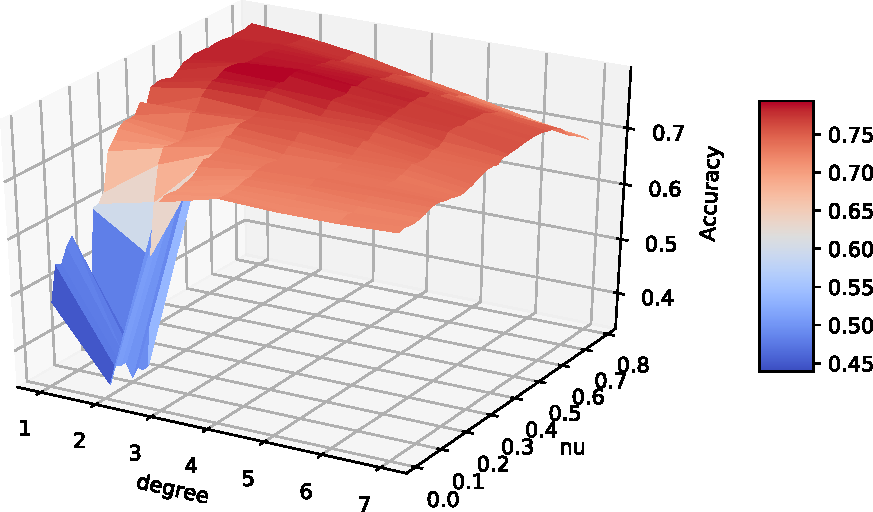
\includegraphics{imgs/poly-no-preprocessing_accuracy.pdf}
\caption{Validation accuracy in a grid search in the two dimensional
space of \(\nu \in [0.02,0,8]\) and \(degree \in [1,7]\). Preprocessing
step: No preprocessing \label{poly-no-preprocessing_accuracy}}
\end{figure}

\begin{figure}
\centering
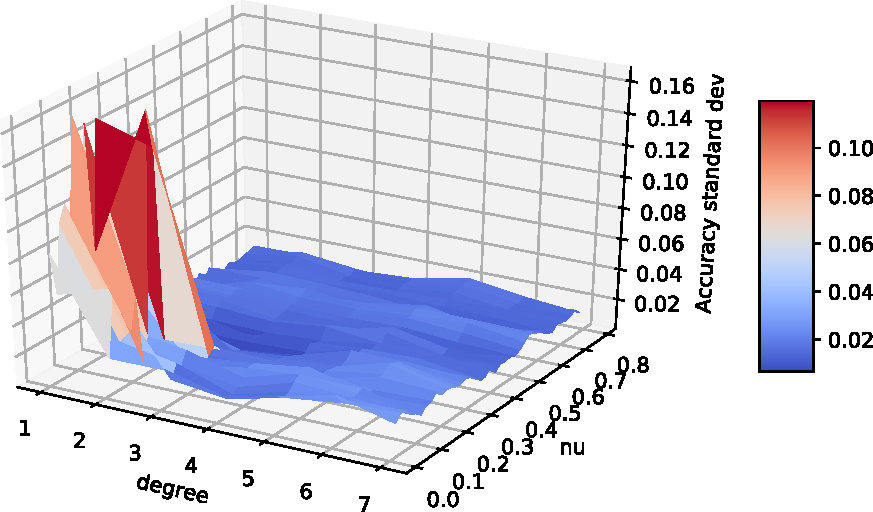
\includegraphics{imgs/poly-no-preprocessing_accuracy_std.pdf}
\caption{Standard deviation of validation accuracy (using 5-fold
crossvalidation) in a grid search in the two dimensional space of
\(\nu \in [0.02,0,8]\) and \(degree \in [1,7]\)
\label{poly-no-preprocessing_accuracy_std}}
\end{figure}

\begin{figure}
\centering
\includegraphics{imgs/poly-no-preprocessing_test-accuracy_errorbar.pdf}
\caption{Validation accuracy for values of \(\nu \in [0.02,0,8]\) and
\(degree = 2\) \label{poly-no-preprocessing_test-accuracy_errorbar}}
\end{figure}

\begin{figure}
\centering
\includegraphics{imgs/poly-no-preprocessing_support_vectors.pdf}
\caption{Number of support vectors for values of \(\nu \in [0.02,0,8]\)
and \(degree \in [1,7]\) \label{poly-no-preprocessing_support_vectors}}
\end{figure}

\begin{itemize}
  \item[Scaling:] As it can be seen in Figure~\ref{poly-scaling_accuracy}, the accuracy
  depends greatly on the $degree$ of the polynomial kernel! Accuracy is higher for odd
  $degree$ values. The highest mean accuracy is about $78.35\%$ with parameters $\nu = 0.64$
  and $degree = 1$, i.e., the best model using scaling is linear and it's not better than
  no preprocessing.
\end{itemize}

\begin{figure}
\centering
\includegraphics{imgs/poly-scaling_accuracy.pdf}
\caption{Validation accuracy in a grid search in the two dimensional
spaces of \(\nu \in [0.02,0,8]\) and \(degree \in [1,7]\). Preprocessing
step: Scaling \label{poly-scaling_accuracy}}
\end{figure}

\begin{itemize}
  \item[Robust scaling:] As with scaling, the accuracy of the model heavily depends on
  $degree$, see Figure~\ref{poly-robust-scaling_accuracy}. The highest mean accuracy is
  about $78.41\%$ with parameters $\nu = 0.64$ and $degree = 1$, same as with regular
  scaling. The idea of robust scaling is to ignore datapoints that are far from the
  central cluster of data, i.e., outliers. No significative change can be seen between
  scaling and robust scaling.
\end{itemize}

\begin{figure}
\centering
\includegraphics{imgs/poly-robust-scaling_accuracy.pdf}
\caption{Validation accuracy in a grid search in the two dimensional
spaces of \(\nu \in [0.02,0,8]\) and \(degree \in [1,7]\). Preprocessing
step: Robust scaling \label{poly-robust-scaling_accuracy}}
\end{figure}

\begin{itemize}
  \item[Normalizing:] As it can be seen in Figure~\ref{poly-normalization_accuracy}, the
  accuracy behaivor with normalization is very similar to the behaivor of no normalization
  at all. The highest mean accuracy is about $79.58\%$ with parameters $\nu = 0.62$ and
  $degree = 3$. Sadly, the best model using normalization isn't much better than the
  baseline, but the surface is smoother and the error doesn't grow much for big values of
  $\nu$ or $degree$
\end{itemize}

\begin{figure}
\centering
\includegraphics{imgs/poly-normalization_accuracy.pdf}
\caption{Validation accuracy in a grid search in the two dimensional
spaces of \(\nu \in [0.02,0,8]\) and \(degree \in [1,7]\). Preprocessing
step: Normalization \label{poly-normalization_accuracy}}
\end{figure}

\begin{itemize}
  \item[Kernel PCA:] Figure~\ref{poly-kernelPCA_gamma2.2_poly2_accuracy} shows the mean
  validation accuracy. The highest mean accuracy is about $79.53\%$ with parameters $\nu =
  0.48$ and $degree = 1$. Sadly, the best model using Kernel PCA isn't much better than
  the baseline. Interestingly, the behaivor of the accuracy for Kernel PCA depends, as
  scaling does, on the degree of the polynomial.
\end{itemize}

\begin{figure}
\centering
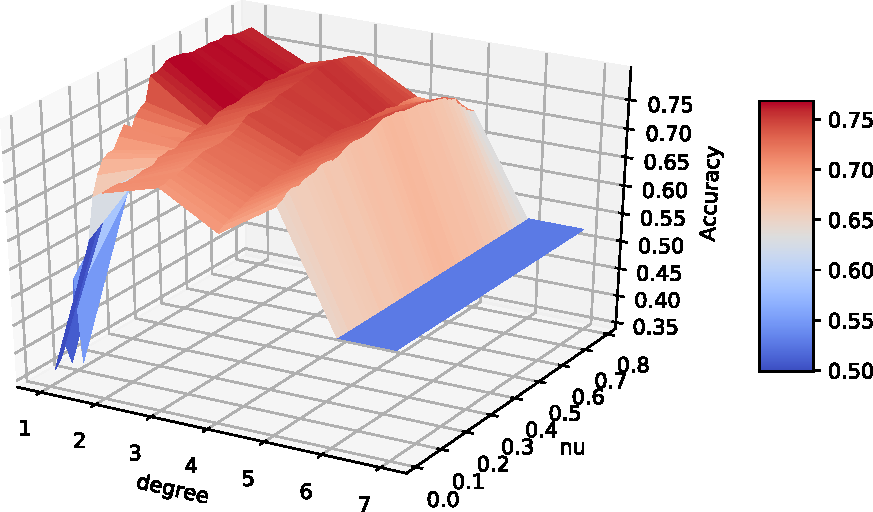
\includegraphics{imgs/poly-kernelPCA_gamma2.2_poly2_accuracy.pdf}
\caption{Validation accuracy in a grid search in the two dimensional
spaces of \(\nu \in [0.02,0,8]\) and \(degree \in [1,7]\). Preprocessing
step: Kernel PCA \label{poly-kernelPCA_gamma2.2_poly2_accuracy}}
\end{figure}

\begin{itemize}
  \item[Autoencoder:] This was my last try in the search of a good preprocessing procedure,
  and it failed terribly. Figure~\ref{poly-autoencoder_accuracy} shows the mean validation
  accuracy. The highest mean accuracy is about $56.00\%$ with parameters $\nu = 0.78$ and
  $degree = 4$, i.e., no good model could be found when compressing the data from 15
  features to 10 using an autoencoder. Figure~\ref{poly-autoencoder_accuracy_std} shows the
  standard deviation for each 5-fold crossvalidation on the grid. All values for the
  standard deviation are low, which means that no matter which values of $\nu$ and
  $degree$ we use, we will always get very bad classification results.
\end{itemize}

\begin{figure}
\centering
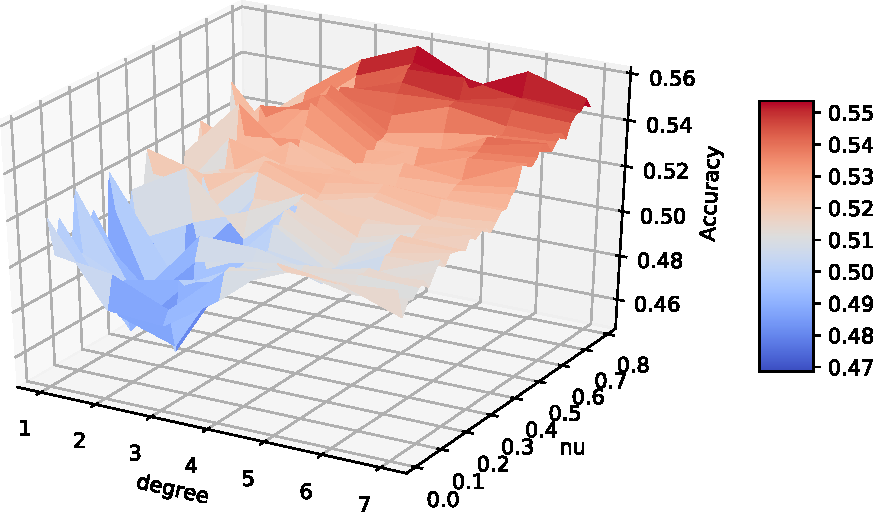
\includegraphics{imgs/poly-autoencoder_accuracy.pdf}
\caption{Validation accuracy in a grid search in the two dimensional
spaces of \(\nu \in [0.02,0,8]\) and \(degree \in [1,7]\). Preprocessing
step: Autoencoder \label{poly-autoencoder_accuracy}}
\end{figure}

\begin{figure}
\centering
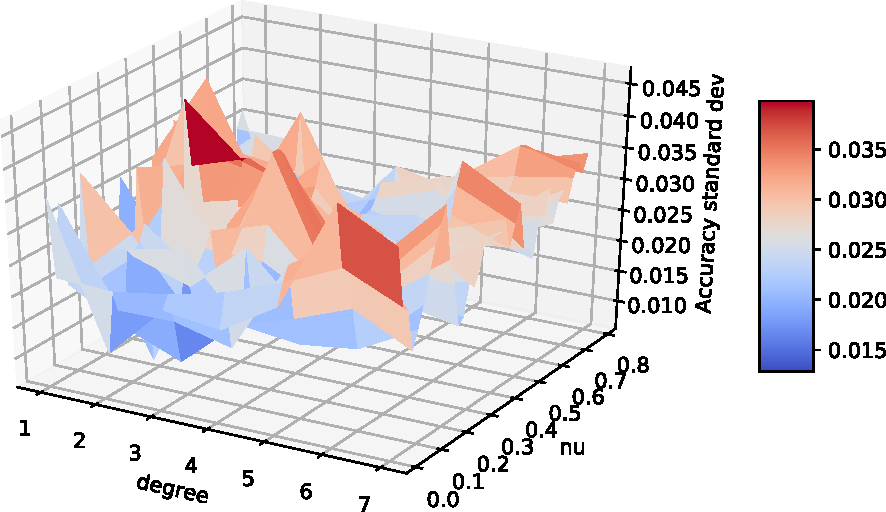
\includegraphics{imgs/poly-autoencoder_accuracy_std.pdf}
\caption{Standard deviation of validation accuracy (using 5-fold
crossvalidation) in a grid search in the two dimensional space of
\(\nu \in [0.02,0,8]\) and \(degree \in [1,7]\)
\label{poly-autoencoder_accuracy_std}}
\end{figure}

The model selected with polynomial kernel is \(\nu = 0.62\) and
\(degree = 3\) with a preprocessing step of normalization.

\subsubsection{Grid search and model selected for gaussian
kernel}\label{grid-search-and-model-selected-for-gaussian-kernel}

Below I present the analysis of the different preprocessing strategies
in the search of the best classification:

\begin{itemize}
  \item[No-preprocessing:] Figure~\ref{rbf-no-preprocessing_accuracy} shows the mean
  validation accuracy with variable values of $\nu \in [0.02,0,8]$ and $\gamma \in
  \{$2.22e-06, 4e-06, 7.2e-06, 1.3e-05, 2.33e-05, 4.2e-05, 7.56e-05, 0.000136, 0.000245,
  0.000441, 0.000793, 0.00143, 0.00257, 0.00463, 0.00833, 0.015, 0.027, 0.0486, 0.0874,
  0.157$\}$. The maximum validation accuracy is around $81.12\%$ with values $\nu = 0.52$ and
  $\gamma = 1.30 \times 10^{-5}$. This validation accuracy is no much bigger than the
  baseline but it improves by more than $1\%$ the mean accuracy, something that couldn't
  be done with the polynomial kernel.

  Figure~\ref{rbf-no-preprocessing_accuracy_std} shows the standard deviation (from the
  5-fold crossvalidation) for each $\nu$ and $\gamma$ in the grid search. The standard
  deviation is low ($<5\%$) for all values were the validation accuracy is high, i.e., for
  values with low mean validation accuracy ($\nu \in [0.02,0.30]$ and $\gamma < 2.45 \times 10^{-4}$)
  their standard deviation is very high, we shouldn't be too confident with those
  values.

  We can see in Figure~\ref{rbf-no-preprocessing_support_vectors} the number of support
  vectors that the final model has. The paramater $\gamma$ influences greatly (more than
  what $degree$ influences the polynomial kernel) the number of support vectors, in fact,
  as it can be seen in Figure~\ref{rbf-no-preprocessing_accuracy_training}, for big values
  of $\gamma$ the model overfits. Notice the highest value on the validation set does not
  fall inside the overfitting zone, which is tranquilizing.
\end{itemize}

\begin{figure}
\centering
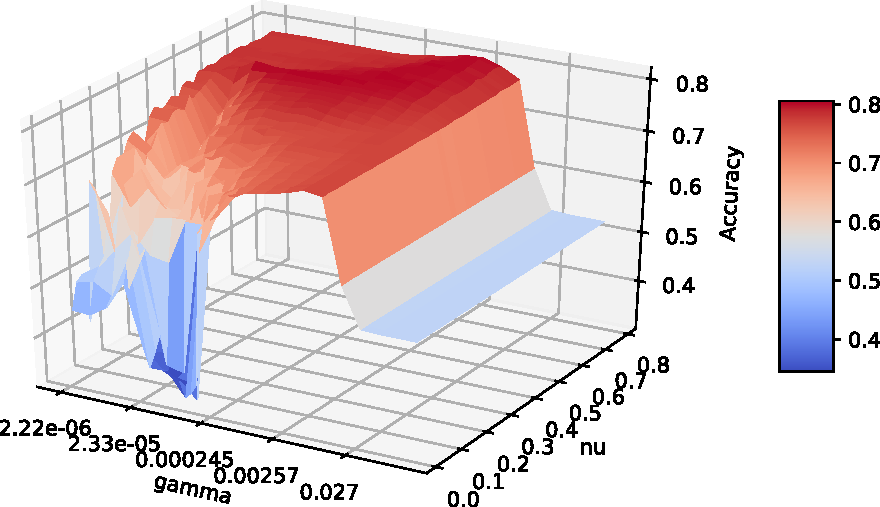
\includegraphics{imgs/rbf-no-preprocessing_accuracy.pdf}
\caption{Validation accuracy in a grid search in the two dimensional
space of \(\nu \in [0.02,0,8]\) and
\(\gamma \in [2.22\times{}10^{-6}, 1.57\times{}10^{-1}]\). Preprocessing
step: No preprocessing \label{rbf-no-preprocessing_accuracy}}
\end{figure}

\begin{figure}
\centering
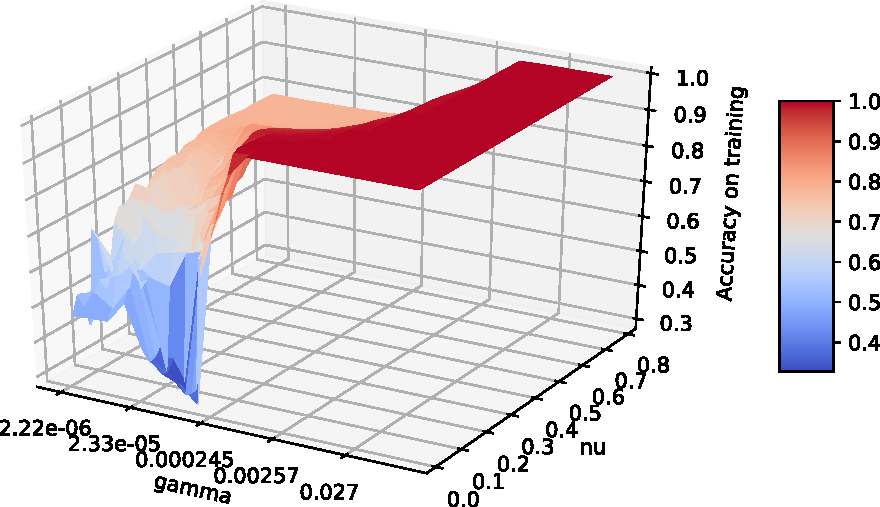
\includegraphics{imgs/rbf-no-preprocessing_accuracy_training.pdf}
\caption{Training accuracy in a grid search in the two dimensional space
of \(\nu \in [0.02,0,8]\) and
\(\gamma \in [2.22\times{}10^{-6}, 1.57\times{}10^{-1}]\). Preprocessing
step: No preprocessing \label{rbf-no-preprocessing_accuracy_training}}
\end{figure}

\begin{figure}
\centering
\includegraphics{imgs/rbf-no-preprocessing_accuracy_std.pdf}
\caption{Standard deviation of validation accuracy (using 5-fold
crossvalidation) in a grid search in the two dimensional space of
\(\nu \in [0.02,0,8]\) and
\(\gamma \in [2.22\times{}10^{-6}, 1.57\times{}10^{-1}]\)
\label{rbf-no-preprocessing_accuracy_std}}
\end{figure}

\begin{figure}
\centering
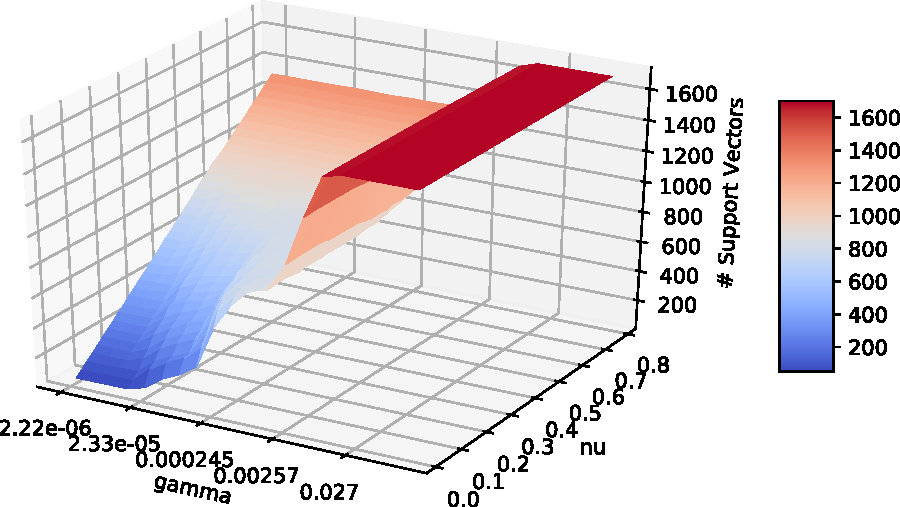
\includegraphics{imgs/rbf-no-preprocessing_support_vectors.pdf}
\caption{Number of support vectors for values of \(\nu \in [0.02,0,8]\)
and \(\gamma \in [2.22\times{}10^{-6}, 1.57\times{}10^{-1}]\)
\label{rbf-no-preprocessing_support_vectors}}
\end{figure}

\begin{itemize}
  \item[Scaling:] Figure~\ref{rbf-scaling_accuracy} shows the mean validation accuracy,
  with $\gamma \in \{$ 4e-05, 7.2e-05, 0.00013, 0.000233, 0.00042, 0.000756, 0.00136,
  0.00245, 0.00441, 0.00793, 0.0143, 0.0257, 0.0463, 0.0833, 0.15, 0.27, 0.486, 0.874,
  1.57, 2.83 $\}$.
  The highest mean accuracy is about $80.65\%$ with parameters $\nu = 0.52$ and $\gamma = 0.00793$.
  The best model using scaling isn't much better than the baseline.
\end{itemize}

\begin{figure}
\centering
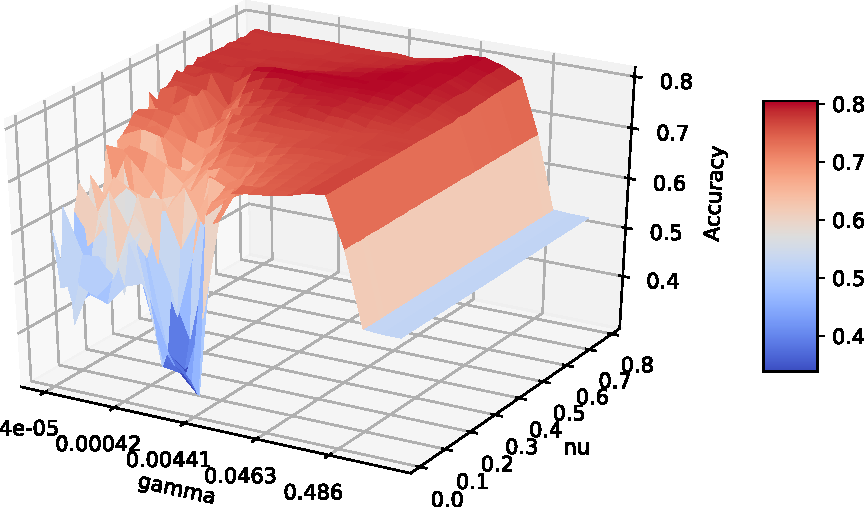
\includegraphics{imgs/rbf-scaling_accuracy.pdf}
\caption{Validation accuracy in a grid search in the two dimensional
spaces of \(\nu \in [0.02,0,8]\) and
\(\gamma \in [4\times{}10^{-5}, 2.83\){]}. Preprocessing step: Scaling
\label{rbf-scaling_accuracy}}
\end{figure}

\begin{itemize}
  \item[Robust scaling:] Figure~\ref{rbf-robust-scaling_accuracy} shows the mean validation accuracy,
  with $\gamma \in \{$ 2e-05, 3.6e-05, 6.48e-05, 0.000117, 0.00021, 0.000378, 0.00068,
  0.00122, 0.0022, 0.00397, 0.00714, 0.0129, 0.0231, 0.0416, 0.075, 0.135, 0.243, 0.437,
  0.787, 1.42 $\}$.
  The highest mean accuracy is about $80.71\%$ with parameters $\nu = 0.52$ and $\gamma = 0.00397$.
  The best model using scaling isn't much better than the baseline. Again as with
  polynomial kernels, robust scaling doesn't change the result of the validation accuracy.
\end{itemize}

\begin{figure}
\centering
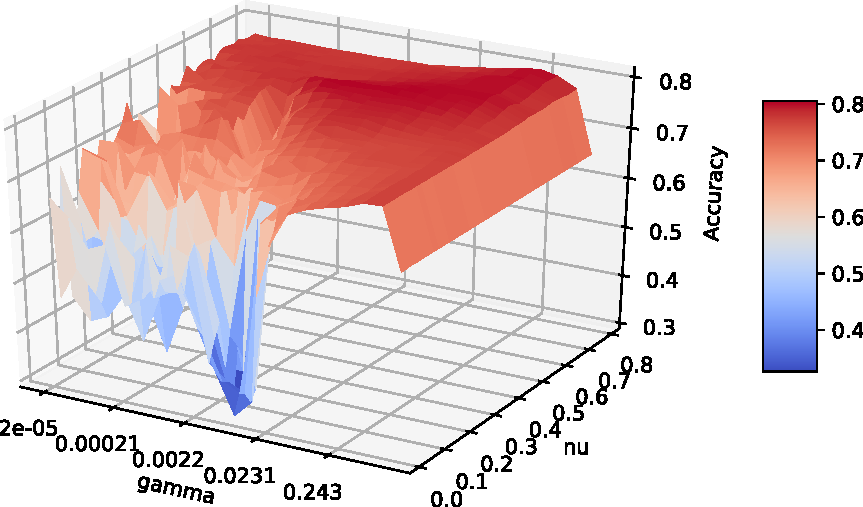
\includegraphics{imgs/rbf-robust-scaling_accuracy.pdf}
\caption{Validation accuracy in a grid search in the two dimensional
spaces of \(\nu \in [0.02,0,8]\) and
\(\gamma \in [2\times{}10^{-5}, 1.42]\). Preprocessing step: Robust
Scaling \label{rbf-robust-scaling_accuracy}}
\end{figure}

\begin{itemize}
  \item[Normalization:] Figure~\ref{rbf-normalization_accuracy} shows the mean validation accuracy,
  with $\gamma \in \{$ 2.44e-05, 5.38e-05, 0.000118, 0.00026, 0.000573, 0.00126, 0.00277,
  0.0061, 0.0134, 0.0295, 0.0649, 0.143, 0.314, 0.691, 1.52, 3.35, 7.36, 16.2, 35.6, 78.4 $\}$.
  The highest mean accuracy is about $79.76\%$ with parameters $\nu = 0.56$ and $\gamma = 0.314$.
  The best model using scaling isn't much better than the baseline. Contrary to the
  polynomial kernel case, normalizing the data before feeding it to training results in
  not the best results.
\end{itemize}

\begin{figure}
\centering
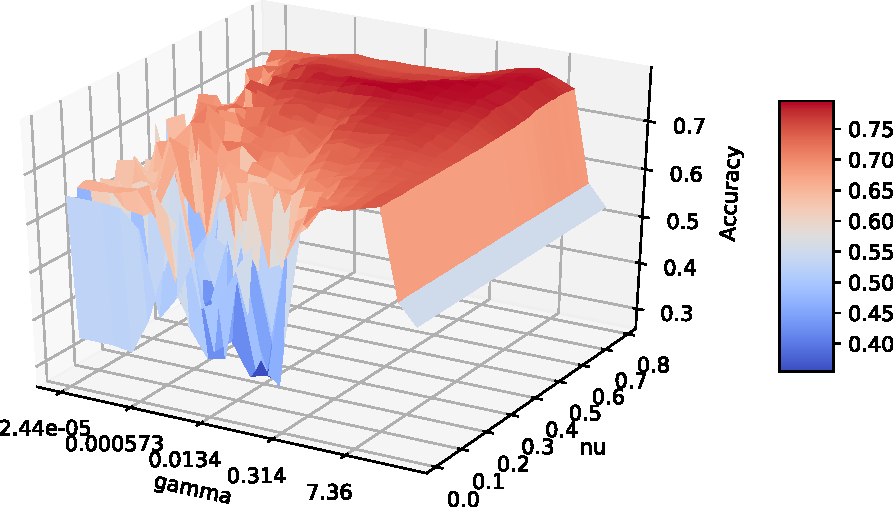
\includegraphics{imgs/rbf-normalization_accuracy.pdf}
\caption{Validation accuracy in a grid search in the two dimensional
spaces of \(\nu \in [0.02,0,8]\) and
\(\gamma \in [2.45\times{}10^{-5}, 78.4]\). Preprocessing step:
Normalizing \label{rbf-normalization_accuracy}}
\end{figure}

\begin{itemize}
  \item[Kernel PCA:] Figure~\ref{rbf-kernelPCA_gamma2.2_poly2_accuracy} shows the mean validation accuracy,
  with $\gamma \in \{$ 1.11e-05, 2.44e-05, 5.38e-05, 0.000118, 0.00026, 0.000573, 0.00126,
  0.00277, 0.0061, 0.0134, 0.0295, 0.0649, 0.143, 0.314, 0.691, 1.52, 3.35, 7.36, 16.2,
  35.6 $\}$.
  The validation accuracy is always the same because it was not possible to learn from the
  data, this was a surprise to me, I still don't understand why it didn't learn anything.
\end{itemize}

\begin{figure}
\centering
\includegraphics{imgs/rbf-kernelPCA_gamma2.2_poly2_accuracy.pdf}
\caption{Validation accuracy in a grid search in the two dimensional
spaces of \(\nu \in [0.02,0,8]\) and
\(\gamma \in [1.11\times{}10^{-5}, 35.6]\). Preprocessing step: Kernel
PCA \label{rbf-kernelPCA_gamma2.2_poly2_accuracy}}
\end{figure}

\begin{itemize}
  \item[Autoencoder:] Figure~\ref{rbf-autoencoder_accuracy} shows the mean validation accuracy,
  with $\gamma \in \{$ 1.11e-05, 2.44e-05, 5.38e-05, 0.000118, 0.00026, 0.000573, 0.00126,
  0.00277, 0.0061, 0.0134, 0.0295, 0.0649, 0.143, 0.314, 0.691, 1.52, 3.35, 7.36, 16.2,
  35.6 $\}$.
  The highest mean accuracy is about $54.82\%$ with parameters $\nu = 0.76$ and $\gamma = 0.000118$.
\end{itemize}

\begin{figure}
\centering
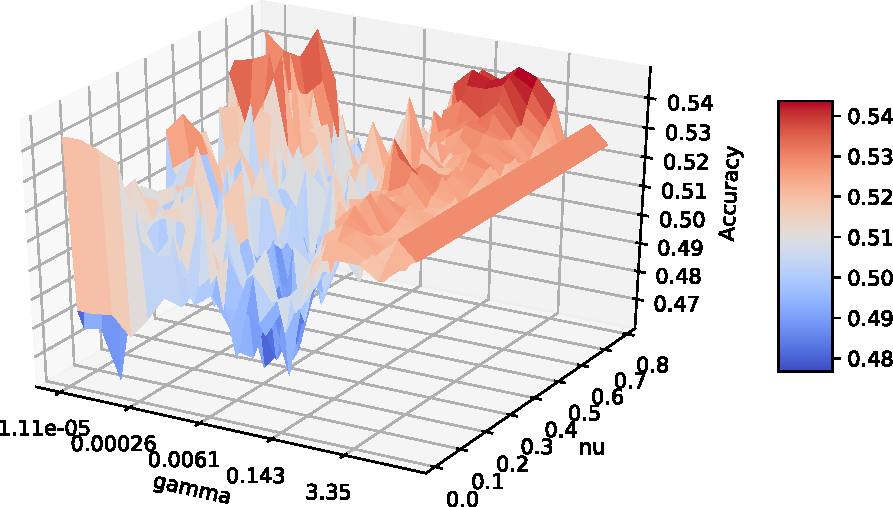
\includegraphics{imgs/rbf-autoencoder_accuracy.pdf}
\caption{Validation accuracy in a grid search in the two dimensional
spaces of \(\nu \in [0.02,0,8]\) and
\(\gamma \in [1.11\times{}10^{-5}, 35.6]\). Preprocessing step:
Autoencoder \label{rbf-autoencoder_accuracy}}
\end{figure}

The model selected with polynomial kernel is \(\nu = 0.52\) and
\(\gamma = 1.30 \times 10^{-5}\) with no preprocessing.

\subsection{Second Problem}\label{second-problem-1}

As explained in subsection\textasciitilde{}\ref{second-problem}
(Preprocessing / Second Problem), I selected two preprocessing
procedures. For each one of them I search in a grid fashion to find the
best parameters, \(\nu\) and \(\lambda\) for the problem\footnote{Once I
  had computed all Gramm matrices for each \(\lambda = \{\) 0.1, 0.2,
  0.3, 0.4, 0.5, 0.6, 0.7, 0.8, 0.9, 1.0 \(\}\), I just computed the
  resulting models of traninig SVMs on several different \(\nu\) values.}.

The results of training the SVMs by preprocessing strategy:

\begin{itemize}
  \item[No preprocessing:] Figure~\ref{no-preprocessing_accuracy} shows the mean
  validation accuracy in the grid search. The highest accuracy value in the search
  corresponds to $89.73\%$ with the parameters $\nu = 0.26$ and $\lambda = 0.6$.

  The standard deviation for each 5-fold crossvalidation is very low, less than $0.5\%$, as
  it can be seen in Figure~\ref{no-preprocessing_accuracy_std}. As with the first problem,
  low values of $\nu$ and $\lambda$ makes for a not so good resulting model.

%  The number of support vectors increases as the value of $\lambda$ does, see
%  Figure~\ref{no-preprocessing_support_vectors}.

  \item[Tokenizing:] Figure~\ref{tokenized_leximized_accuracy} shows the mean
  validation accuracy in the grid search. The highest accuracy value in the search
  corresponds to $91.20\%$ with the parameters $\nu = 0.2$ and $\lambda = 0.55$. The
  behaivor of lists of tokens (one per word) is radically different to the behaivor of
  lists of characters, but their computation times are the same once the kernels have been
  computed.

  The standard deviation for each 5-fold crossvalidation is very-very low, less than
  $0.25\%$! see Figure~\ref{tokenized_leximized_accuracy_std}. The standard deviation with
  this preprocessing beats applying no preprocessing at all, this preprocessing procedure
  seems to be superior.
\end{itemize}

\begin{figure}
\centering
\includegraphics{imgs/no-preprocessing_accuracy.pdf}
\caption{Validation accuracy in a grid search in the two dimensional
spaces of \(\nu \in [0.02,0,8]\) and \(\lambda \in [0.1, 1.0]\).
Preprocessing step: No preprocessing \label{no-preprocessing_accuracy}}
\end{figure}

\begin{figure}
\centering
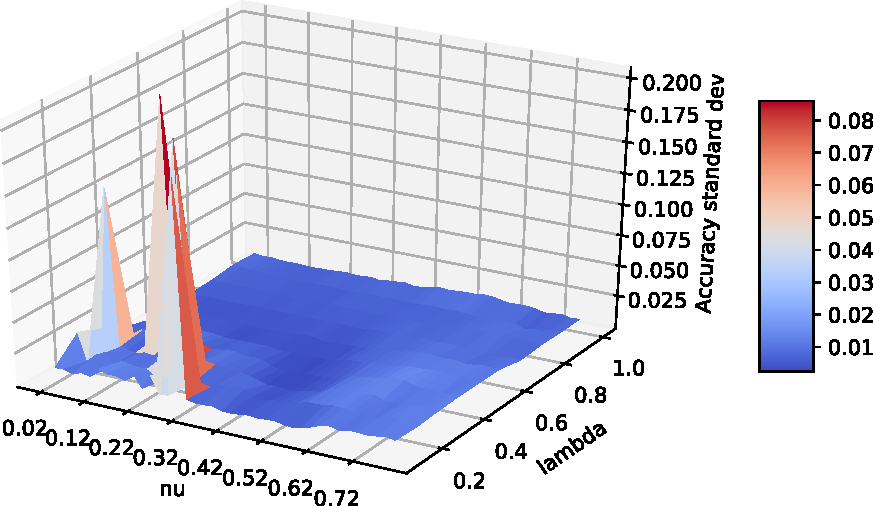
\includegraphics{imgs/no-preprocessing_accuracy_std.pdf}
\caption{Standard deviation of validation accuracy (using 5-fold
crossvalidation) in a grid search in the two dimensional space of
\(\nu \in [0.02,0,8]\) and \(\lambda \in [0.1, 1.0]\).
\label{no-preprocessing_accuracy_std}}
\end{figure}

\begin{figure}
\centering
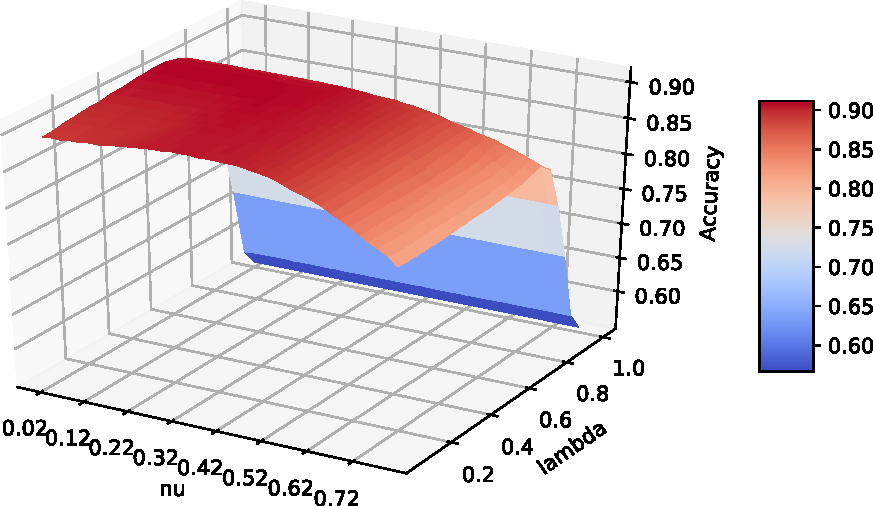
\includegraphics{imgs/tokenized_leximized_accuracy.pdf}
\caption{Validation accuracy in a grid search in the two dimensional
spaces of \(\nu \in [0.02,0,8]\) and \(\lambda \in [0.1, 1.0]\).
Preprocessing step: Tokenized and Leximized
\label{tokenized_leximized_accuracy}}
\end{figure}

\begin{figure}
\centering
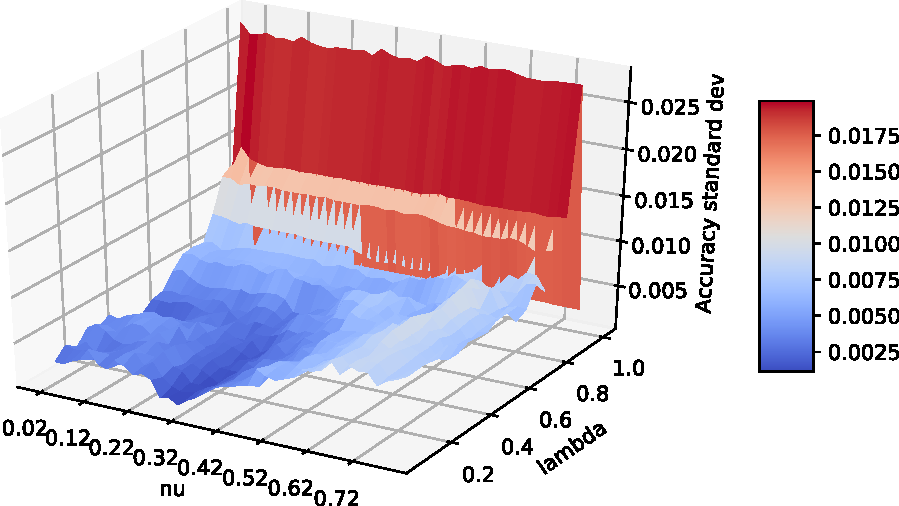
\includegraphics{imgs/tokenized_leximized_accuracy_std.pdf}
\caption{Standard deviation of validation accuracy (using 5-fold
crossvalidation) in a grid search in the two dimensional space of
\(\nu \in [0.02,0,8]\) and \(\lambda \in [0.1, 1.0]\).
\label{tokenized_leximized_accuracy_std}}
\end{figure}

The model selected corresponds to the one obtained applying
\(\nu = 0.2\) and \(\lambda = 0.55\) with Tokenizing and Lemmatizing as
preprocessing.

\section{Training and Analysis}\label{training-and-analysis}

\subsection{First Problem}\label{first-problem-2}

\subsubsection{Polynomial Kernel}\label{polynomial-kernel}

The testing accuracy for the model selected (\(\nu = 0.62\) and
\(degree = 3\) with normalization) is of 81.00\%, a better value than
79.58\% that was obtained with less datapoints (validation datapoints),
therefore it seems accurate to say that the real accuracy value for the
model is about 81.00\%, but remember that this value is highly
expeculative because, as we know from
subsection\textasciitilde{}\ref{first-problem} (Preprocessing / First
Problem), because with a test set of only 300 datapoints the estimation
could be off up to 7.8\%. Therefore the real value lies between
\([73.2\% , 88.8\%]\), but I am hopeful that the actual accuracy will
fall very close to 81.00\% with an error of about 4\% (not 7.8\%).

\subsubsection{Gaussian Kernel}\label{gaussian-kernel}

The testing accuracy for the model selected (\(\nu = 0.52\) and
\(\gamma = 1.30 \times 10^{-5}\)) is of 80.67\%, marginally better than
the original model trained with less datapoints. Given the size of the
test set (300), the actual accuracy for the model lies between
\([ 72.87\%, 88.47\%]\), but given that the accuracy measure didn't
change much with more data I adventure to say that the error between the
real accuracy and the one from the testing data isn't more than 4\%.

\subsection{Second Problem}\label{second-problem-2}

The testing accuracy for the model (\(\nu = 0.2\) and
\(\lambda = 0.55\)) is \(90.79\%\), which is lower to the result gotten
in the k-fold crossvalidation. The real accuracy value falls between
\([87.44\%, 94.14\%]\) with a confidence of 95\%.

It is very interesting though, how well the binary classifier works with
some preprocessing. The preprocessing procedure reduces greatly the
amount of work to compute the kernels but it also gives better results
than pure kernels in strings. This may be because the lexemizer used
groups many words by their semantic meanings, and that added information
helps the process of differenciating between two types of news greatly.

\section{Conclusions}\label{conclusions}

The two problems were easy to solve but required big amounts of
computing time to find the right models, the right (hype-)parameters.
This is specially true for the second problem, which required storing in
memory almost a gigabyte, and took 14 hours to compute a single gramm
matrix to feed into an SVM optimizer.

SVMs are very powerful, but they require the hard task of finding the
right kernel for a task, the more complex a kernel is the more
information it has about a specific problem, but the harder it gets to
compute, and therefore the computation time gets higher.

At first SVMs seemed mystical, those things that the industry used to
use heavily, but are they hard to use? Not really, many packages for
machine learning come with them included, and they are quite fast to
calculate for small amounts of data (few thousend). Their major drawback
is that computing using big amounts of data seems to be a little hard,
or at least at little annoying.

\section{Appendix}\label{appendix}

The second problem required the use of a kind of ``obscure'' kernel for
strings, namely String Subsequences Kernel (SSK) and the only
implementation available was that of shogun (Sonnenburg et al.
\protect\hyperlink{ref-shogun_2017}{2017}). Shogun has one huge
drawback, it is rather un-pythonic, its API hasn't been designed to
integrate cleanly with python idioms or ways of passing around objects.
Besides, it seems like shogun doesn't have best support for installation
in any platform, the best way to install it is by compiling it from
source, which I managed to do, but didn't feel as worthed to anyone else
who wanted to use the code I've written.

I, therefore, implemented the fast-SSK subroutine presented in Lodhi et
al. (\protect\hyperlink{ref-lodhi2002text}{2002}). The naive recursive
version shown in the paper is rather slow, a very efficient version of
the algorithm can be written by transforming all recursions into loops,
and managing caching efficiently. In the end, after some optimizations I
arrived to a similar perfromant version of the algorithm developed in
shogun, but I want to clarify two things: first, I took a clever idea
from the shogun implementation, and second, the algorithm is written in
Cython not python, the python version is hundreds of times slower than
the Cython version, this is given to all the stuff python does on
runtime, checking the types and other things.

The code to the implementation SSK can be found in
\url{https://github.com/helq/python-ssk} with CC0 license (Public Domain
Dedication).

\section*{References}
\setlength{\parindent}{-0.2in}
\singlespacing
\small
\setlength{\leftskip}{0.2in}
\setlength{\parskip}{8pt}
\vspace*{-0.4in}
\noindent

\hypertarget{refs}{}
\hypertarget{ref-BirdKleinLoper09}{}
Bird, Steven, Ewan Klein, and Edward Loper. 2009. \emph{Natural Language
Processing with Python}. O'Reilly Media.

\hypertarget{ref-wordnet}{}
Fellbaum, Christiane. 1998. \emph{WordNet: An Electronic Lexical
Database}. Bradford Books.

\hypertarget{ref-lodhi2002text}{}
Lodhi, Huma, Craig Saunders, John Shawe-Taylor, Nello Cristianini, and
Chris Watkins. 2002. ``Text Classification Using String Kernels.''
\emph{Journal of Machine Learning Research} 2 (Feb): 419--44.

\hypertarget{ref-scikit-learn}{}
Pedregosa, F., G. Varoquaux, A. Gramfort, V. Michel, B. Thirion, O.
Grisel, M. Blondel, et al. 2011. ``Scikit-Learn: Machine Learning in
Python.'' \emph{Journal of Machine Learning Research} 12: 2825--30.

\hypertarget{ref-shogun_2017}{}
Sonnenburg, Soeren, Heiko Strathmann, Sergey Lisitsyn, Viktor Gal,
Fernando J. Iglesias García, Wu Lin, Soumyajit De, et al. 2017.
``Shogun-Toolbox/Shogun: Shogun 6.0.0 - Baba Nobuharu,'' April. Zenodo.
doi:\href{https://doi.org/10.5281/zenodo.556748}{10.5281/zenodo.556748}.

\end{document}
